% Propósito: mostrar que presión y velocidad de partícula están en fase en una
% onda plana progresiva, mientras la intensidad instantánea es su producto.
% Origen: p=p_hat sin(omega t), u=u_hat sin(omega t) e
% i=p_hat u_hat sin^2(omega t), bajo las hipótesis de la
% ecuación \eqref{eq:u4-impedancia-caracteristica}.
% Curvas teóricas normalizadas; no representan datos medidos.
% Descripción accesible: tres gráficos comparten un período. La presión y la
% velocidad normalizadas tienen la misma forma sinusoidal y cruzan cero a la
% vez. La intensidad normalizada es siempre no negativa y presenta dos máximos
% por período, lo que indica flujo neto de energía en la dirección de avance.
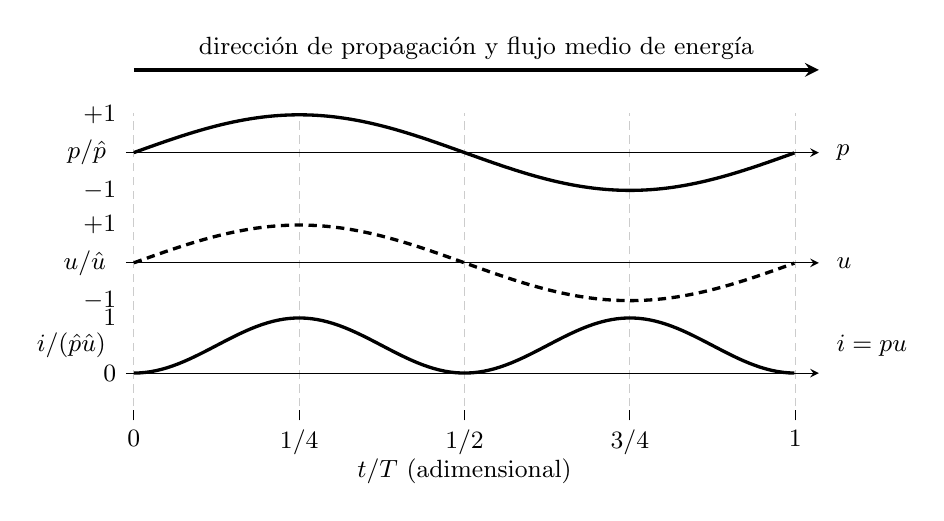
\begin{tikzpicture}[font=\small,>=stealth,x=1cm,y=1cm]
    \draw[->,very thick] (2.15,4.20) -- (10.85,4.20)
        node[midway,above] {dirección de propagación y flujo medio de energía};

    \foreach \q/\lab in {0/{0},0.25/{1/4},0.5/{1/2},0.75/{3/4},1/{1}}{
        \pgfmathsetmacro{\xx}{2.15+8.4*\q}
        \draw[densely dashed,black!20] (\xx,-0.25) -- (\xx,3.65);
        \draw (\xx,-0.25) -- (\xx,-0.12);
        \node[below] at (\xx,-0.25) {\(\lab\)};
    }

    \foreach \yy in {3.15,1.75,0.35}{
        \draw[->] (2.05,\yy) -- (10.85,\yy);
    }

    \node[anchor=east] at (1.92,3.15) {\(p/\hat p\)};
    \node[anchor=east] at (1.92,1.75) {\(u/\hat u\)};
    \node[anchor=east,align=right] at (1.92,0.70)
        {\(i/(\hat p\hat u)\)};

    \node[anchor=east] at (2.05,3.63) {\(+1\)};
    \node[anchor=east] at (2.05,2.67) {\(-1\)};
    \node[anchor=east] at (2.05,2.23) {\(+1\)};
    \node[anchor=east] at (2.05,1.27) {\(-1\)};
    \node[anchor=east] at (2.05,1.05) {\(1\)};
    \node[anchor=east] at (2.05,0.35) {\(0\)};

    \draw[very thick,samples=120,domain=0:1]
        plot ({2.15+8.4*\x},{3.15+0.48*sin(360*\x)});
    \draw[very thick,densely dashed,samples=120,domain=0:1]
        plot ({2.15+8.4*\x},{1.75+0.48*sin(360*\x)});
    \draw[very thick,samples=120,domain=0:1]
        plot ({2.15+8.4*\x},{0.35+0.70*(sin(360*\x))^2});

    \node[anchor=west] at (10.95,3.15) {\(p\)};
    \node[anchor=west] at (10.95,1.75) {\(u\)};
    \node[anchor=west] at (10.95,0.70) {\(i=pu\)};
    \node at (6.35,-0.90) {\(t/T\) (adimensional)};
\end{tikzpicture}
